\section{Solución}\label{sec:solution}

En esta sección se describe el algoritmo utilizado para resolver el problema planteado.
Al mismo tiempo, se explican los pasos que se deben seguir para poder ejecutar el programa.
Así como un ejemplo de ejecución del programa utilizando una imagen de prueba.

% Preparación del ambiente

\subsection{Preparación del ambiente}\label{subsec:environment-preparation}

Para poder ejecutar el programa, se debe tener instalado el compilador de C++ \texttt{g++} y la herramienta \texttt{make}.
Además, se debe tener instalado el paquete \texttt{libopencv-dev} para poder utilizar la librería \texttt{OpenCV}.

Para instalar \texttt{libopencv-dev}, se debe ejecutar el Comando~\ref{lst:install_opencv}.
\begin{lstlisting}[float=H,caption={Install OpenCV},label={lst:install_opencv}]
sudo apt-get install libopencv-dev
\end{lstlisting}

% Compilación

\subsubsection{Compilación}\label{subsubsec:compilation}

Para compilar el programa, se debe ejecutar el Comando~\ref{lst:compile}.
\begin{lstlisting}[float=H,caption={Compilation},label={lst:compile}]
make
\end{lstlisting}

% Ejecución

\subsubsection{Ejecución}\label{subsubsec:execution}

El programa tiene un parámetro opcional, que es el nombre de la imagen a utilizar.
Si no se especifica el nombre de la imagen, se utilizará una imagen por defecto.
Que es una imagen de prueba de 3x3.

Para ejecutar el programa, se debe ejecutar el siguiente comando:
\begin{lstlisting}[float=H,caption={Ejecution},label={lst:run}]
./main [image_name]
\end{lstlisting}

% Algoritmo

\subsection{Algoritmo}\label{subsec:algorithm}

\subsubsection{Importar imagen}\label{subsubsec:import-image}
Importar imagen a color en formato CIE-Lab.

Para esto se utiliza la Función~\ref{lst:load_image}.

\begin{lstlisting}[float=H,caption={Load Image},label={lst:load_image}]
void ImageRepo::byName(
    Mat &image,
    Mat &imageOriginal,
    const string &name
    ) {
    // Read image.
    imageOriginal = imread(name);
    // Convert to float values.
    Mat imageFloat;
    imageOriginal.convertTo(imageFloat, CV_32FC3);
    // Normalize.
    imageFloat /= 255.0;
    // Convert to BGR2Lab.
    cvtColor(imageFloat, image, COLOR_BGR2Lab);
}
\end{lstlisting}

En este ejemplo, se utilizará la imagen de la Figura~\ref{fig:test_img_3x3}.

\begin{figure}[H]
    \centering
    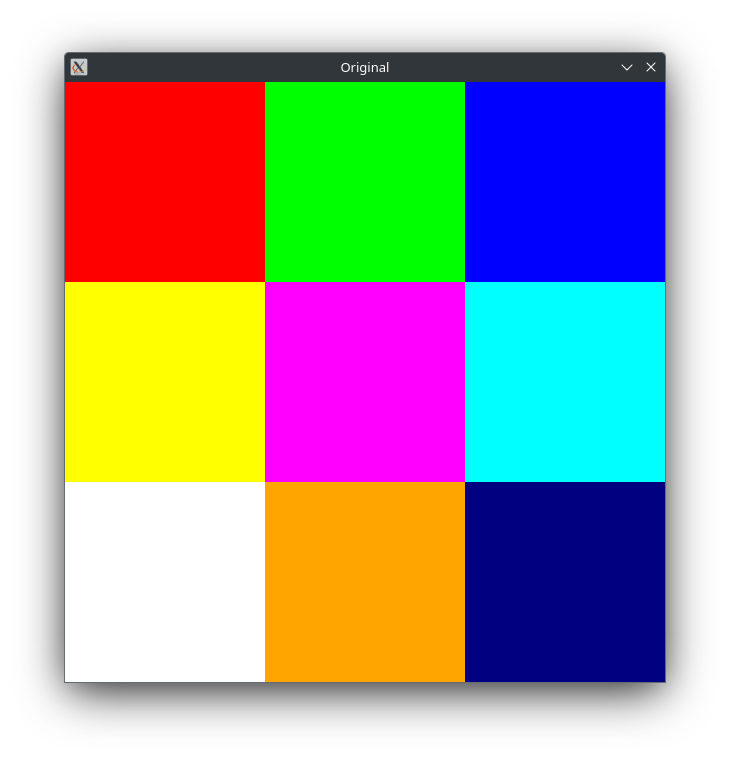
\includegraphics[width=.3\textwidth]{./latex/img/original}
    \caption{Imagen de prueba de 3x3.}
    \label{fig:test_img_3x3}
\end{figure}

\subsubsection{Generar máscara}\label{subsubsec:generate-mask}
Se genera una máscara de la misma dimensión que la imagen, que contiene las clases a las que pertenece cada pixel.
(Inicialmente, todos los píxeles pertenecen a la misma clase \("0"\) ).
El Código~\ref{lst:init_mask} muestra como se inicializa la máscara.

\begin{lstlisting}[float=H,caption={Compilation},label={lst:init_mask}]
// init mask with zeros.
mask = Mat::zeros(image.size(), CV_8UC1);
\end{lstlisting}

Al inicializar la máscara, todos los píxeles pertenecen a la misma clase, por lo que la máscara se inicializa con todos los píxeles con el valor 0.
La máscara es la siguiente matriz:

\begin{equation*}
    \begin{bmatrix}
        0 & 0 & 0 \\
        0 & 0 & 0 \\
        0 & 0 & 0
    \end{bmatrix}
\end{equation*}

\subsubsection{Calcular estadísticas}\label{subsubsec:calculate-statistics}

Ahora se procede a calcular las estadísticas (vector promedio y matriz de covarianza) de cada clase.
(Como solo existe la clase 0, se calculan solo las estadísticas de esta clase).


Para esto se utiliza la Función~\ref{lst:mean_covariance}.
\begin{lstlisting}[float=H,caption={Mean And Covariance},label={lst:mean_covariance}]
int MatTools::meanCovariance(Mat &image, Mat &mask, map<int, ImageStats> &stats, vector<int> &labels, bool covariance) {
    auto result = MatTools::mean(image, mask, stats, labels);
    if (0 != result) {
        return result;
    }
    if (covariance) {
        // calculate covariance
        auto itMask = mask.begin<uchar>();
        auto itMaskEnd = mask.end<uchar>();
        auto itImage = image.begin<Vec3f>();

        while (itMask != itMaskEnd) {
            auto label = *itMask;
            auto &imageStats = stats[label];
            auto a = (*itImage)[1];
            auto b = (*itImage)[2];
            auto ad = a - imageStats.mean.a;
            auto bd = b - imageStats.mean.b;
            imageStats.covariance.s1 += ad * ad;
            imageStats.covariance.s2 += bd * bd;
            imageStats.covariance.s3 += ad * bd;
            itMask++;
            itImage++;
        }

        for (auto &item: stats) {
            auto &imageStats = item.second;
            auto &count = imageStats.count;
            if (count < 2) {
                continue;
            }
            auto iCont = (float) (1. / (count - 1));
            imageStats.covariance.s1 *= iCont;
            imageStats.covariance.s2 *= iCont;
            imageStats.covariance.s3 *= iCont;
        }

    }
    return 0;
}
\end{lstlisting}

Como se puede observar, las estadísticas se almacenan en un diccionario, donde la clave es el número de la clase y el valor es una estructura de tipo \texttt{ImageStats}.
La estructura \texttt{ImageStats} contiene el vector promedio y la matriz de covarianza de la clase.
Lo podemos ver en Código~\ref{lst:image_stats}.
\begin{lstlisting}[float=H,caption={Image Stats},label={lst:image_stats}]
struct ImageStats {
    // vector of Lab averages
    struct {
        float l = 0;
        float a = 0;
        float b = 0;
    } mean;
    // covariance matrix
    struct {
        float s1 = 1;
        float s2 = 1;
        float s3 = 0;
    } covariance;
    // number of pixels
    int count = 0;
    // class label
    int label = 0;
};
\end{lstlisting}

Siguiendo con el ejemplo, ahora tenemos disponible la media y la matriz de covarianza de la clase 0.

En la Figura~\ref{fig:stats_0}, depuramos el código y podemos ver estas estadísticas:

\begin{figure}[H]
    \centering
    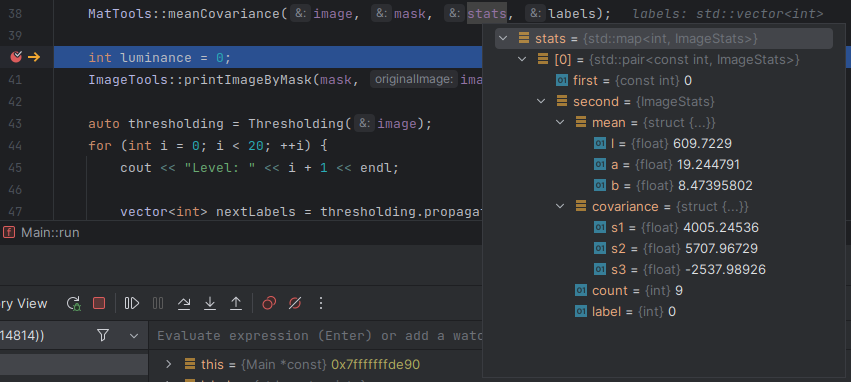
\includegraphics[width=1\textwidth]{./latex/img/stats_0}
    \caption{Estadísticas de la clase 0.}
    \label{fig:stats_0}
\end{figure}

\subsubsection{Construir imagen}\label{subsubsec:build-image}

Ahora, con información de la máscara y las estadísticas podríamos construir una imagen en formato CIE-Lab, donde cada píxel sea el vector promedio de la clase a la que pertenece.

La Figura~\ref{fig:m0} nos muestra la imagen construida con la clase 0.

\begin{figure}[H]
    \centering
    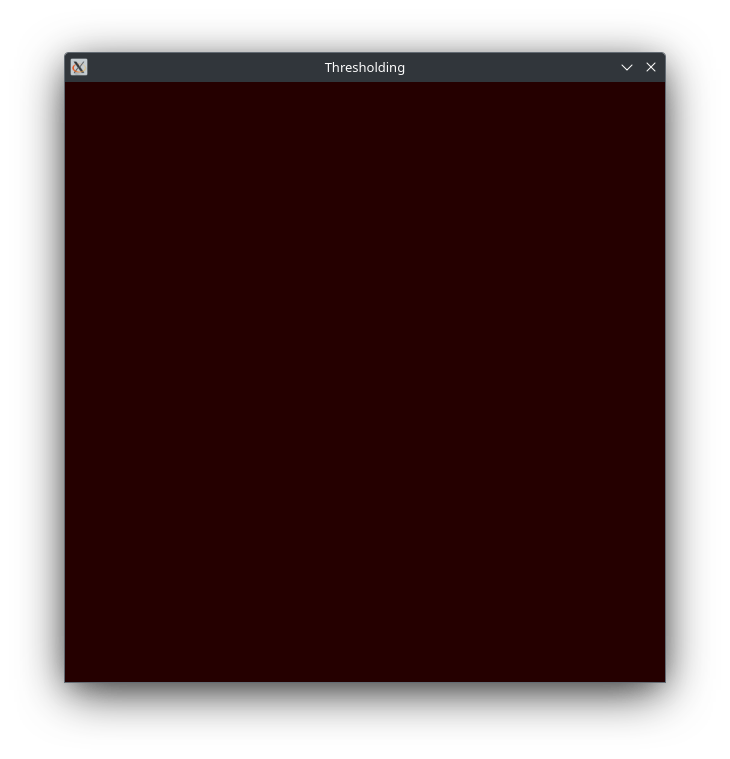
\includegraphics[width=.35\textwidth]{./latex/img/m0}
    \caption{Imagen construida con la clase 0 (Luminosidad: 0).}
    \label{fig:m0}
\end{figure}

Tener en cuenta que la luminosidad de la imagen es 0.
El objetivo de esto es que se vean iguales los pixeles que pertenecen a la misma clase.

\subsubsection{Dividir máscara}\label{subsubsec:split-mask}

Ahora, se procede a dividir la máscara (en este caso la 0) en dos nuevas máscaras (1 y 2).
Esto se realiza con la Función~\ref{lst:divide_class}.

\begin{lstlisting}[float=H,caption={Divide Class},label={lst:divide_class}]
vector<int> Thresholding::divideClass(Mat &mask, int label) {
    int newLabelA = Thresholding::lastLabel++;
    int newLabelB = Thresholding::lastLabel++;
    int changesCount = 0;
    auto it = mask.begin<uchar>();
    auto itEnd = mask.end<uchar>();
    for (; it != itEnd; ++it) {
        if (*it == label) {
            *it = (0 == (changesCount % 2)) ? newLabelA : newLabelB;
            changesCount++;
        }
    }
    return vector<int>({newLabelA, newLabelB});
}
\end{lstlisting}

El cual vemos que pide por parámetro la máscara y la clase a dividir.
Se decidió para este caso ir alternando la asignación de las nuevas clases, de esta forma se garantiza que no se generen clases vacías.
La función devuelve un vector con los dos nuevos labels en un vector de enteros.

\subsubsection{Distancia de Mahalanobis}\label{subsubsec:mahalanobis}

El resultado de la acción anterior nos devuelve una nueva máscara con dos clases.
Pero debemos hacer un proceso de umbralización para determinar agrupar los píxeles en la clase de la que más se acerquen.
Para esto vamos a necesitar una función que nos permita calcular la distancia de Mahalanobis entre un píxel y una clase.
La Función~\ref{lst:mahalanobis} nos permite calcular la distancia de Mahalanobis entre un píxel y una clase.

\begin{lstlisting}[float=H,caption={Mahalanobis Distance},label={lst:mahalanobis}]
double MatTools::distanceMahalanobisNormalized(double a, double b, ImageStats imageStats) {
    auto &mean = imageStats.mean;
    auto &covariance = imageStats.covariance;
    auto ad = a - mean.a;
    auto bd = b - mean.b;
    auto s1 = covariance.s1;
    auto s2 = covariance.s2;
    auto s3 = covariance.s3;
    auto d = (ad * ad) / s1 + (bd * bd) / s2 - 2 * (ad * bd) / s3;

    return ad * ad + bd * bd;
}
\end{lstlisting}

La función recibe como parámetros el píxel a calcular la distancia y la estructura de estadísticas de la clase.

\subsubsection{Reordenar píxeles}\label{subsubsec:reorder-pixels}
Esta función que calcula la Distancia de Mahalanobis será utilizada en la Función~\ref{lst:reorder_pixels} \texttt{reorderPixels} para reordenar los píxeles de la máscara.

\begin{lstlisting}[float=H,caption={Reorder Pixels},label={lst:reorder_pixels}]
int Thresholding::reorderPixels(
        Mat &mask,
        vector<int> &labels,
        map<int, ImageStats> &stats,
        bool &hasClassA,
        bool &hasClassB
) {
    int classA = labels[0];
    int classB = labels[1];
    ImageStats imageStatsClassA = stats[classA];
    ImageStats imageStatsClassB = stats[classB];

    auto itImage = this->image.begin<Vec3f>();
    auto itMask = mask.begin<uchar>();
    auto itEnd = mask.end<uchar>();
    int changesCount = 0;
    while (itMask != itEnd) {
        auto &label = *itMask;
        if (classA != label && classB != label) {
            itImage++;
            itMask++;
            continue;
        }
        Vec3f pixel = *itImage;
        float a = pixel[1];
        float b = pixel[2];
        // Calculate distance.
        double distanceA = MatTools::distanceMahalanobisNormalized(a, b, imageStatsClassA);
        double distanceB = MatTools::distanceMahalanobisNormalized(a, b, imageStatsClassB);
        if (distanceA < distanceB) {
            hasClassA = true;
            if (classA != label) {
                label = classA;
                changesCount++;
            }
        } else {
            hasClassB = true;
            if (classB != label) {
                label = classB;
                changesCount++;
            }
        }
        itImage++;
        itMask++;
    }

    return changesCount;
}
\end{lstlisting}

Esta función recibe por parámetro la máscara, los labels de las clases a reordenar, las estadísticas de las clases y dos variables booleanas que indican si la clase A y la clase B tienen píxeles asignados.

\subsubsection{Umbralizar}\label{subsubsec:thresholding}

Ahora con estas funciones disponibles, podemos proceder a umbralizar la imagen.
La Función~\ref{lst:thresholding} \texttt{toThreshold} es la encargada de realizar el proceso de umbralización.

\begin{lstlisting}[float=H,caption={Mahalanobis Distance},label={lst:thresholding}]
int Thresholding::toThreshold(
        Mat &mask,
        vector<int> &labels,
        map<int, ImageStats> &stats,
        bool &hasClassA,
        bool &hasClassB,
        bool covariance
) {
    int limit = covariance ? iterationsLimitWithConvergence : iterationsLimitWithoutConvergence;
    for (int i = 0; i < limit; i++) {
        cout << "Iteration: " << i << endl;

        hasClassA = false;
        hasClassB = false;

        int classA = labels[0];
        int classB = labels[1];

        cOutImageStats(stats[classA]);
        cOutImageStats(stats[classB]);

        auto changesCount = this->reorderPixels(
                mask,
                labels,
                stats,
                hasClassA,
                hasClassB
        );

        if (0 == changesCount) {
            cout << "El algoritmo convergió en " << i << " iteraciones." << endl;
            return 0;
        } else {
            cout << "Hubo: " << changesCount << " cambios." << endl;
            MatTools::meanCovariance(this->image, mask, stats, labels, covariance);
        }
    }

    return 1;
}
\end{lstlisting}

La función recibe por parámetro la máscara, los labels de las clases a umbralizar, las estadísticas de las clases, dos variables booleanas que indican si la clase A y la clase B tienen píxeles asignados y un booleano que indica si se debe utilizar la covarianza o no.
Este último parámetro es utilizado en las primeras iteraciones para que se utilice la distancia Euclidiana (Mahalanobis sin covarianza) y en las siguientes iteraciones se utilice la distancia de Mahalanobis.

\subsubsection{Primera iteración}\label{subsubsec:first-iteration}

Luego de la umbralización, se obtiene una máscara con dos clases (1 y 2) en la cual, cada clase contiene píxeles más cercanos.

Para el ejemplo que estamos utilizando, la máscara resultante es la siguiente:

\begin{equation*}
    \begin{bmatrix}
        2 & 2 & 1 \\
        2 & 1 & 2 \\
        2 & 2 & 1
    \end{bmatrix}
\end{equation*}

Si construimos la imagen a partir de la máscara, obtenemos la siguiente imagen:
La Figura~\ref{fig:m1} nos muestra la imagen construida con la máscara actual (conformada por las clases 1 y 2).

\begin{figure}[H]
    \centering
    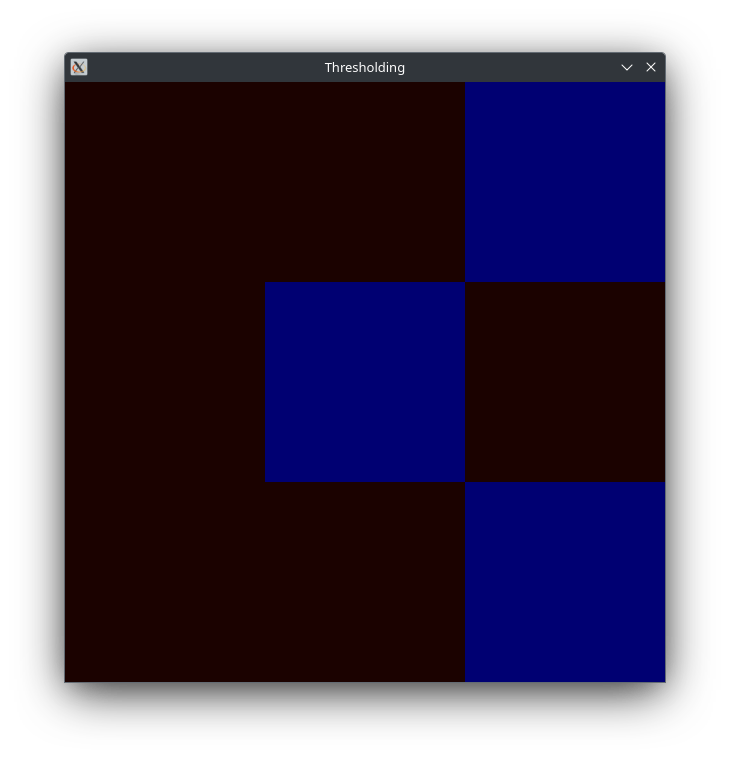
\includegraphics[width=.35\textwidth]{./latex/img/m1}
    \caption{Imagen construida con las clases 1 y 2 (Luminosidad: 0).}
    \label{fig:m1}
\end{figure}

Como podemos observar, todos los píxeles que pertenecen a la clase 1 se observan del mismo color (rojo oscuro) y los píxeles que pertenecen a la clase 2 se observan del mismo color (azul oscuro).

\subsubsection{Propagación}\label{subsubsec:propagation}

Lo siguiente que debemos hacer es continuar iterando para generar más clases y así obtener una imagen con más colores.
En la iteracion siguiente, se espera que se generen para la clase 1, dos clases más (3 y 4) y para la clase 2, dos clases más (5 y 6).
Este proceso se repite hasta que las clases no se puedan dividir más.
La Función~\ref{lst:propagation_fun} \texttt{propagate} se encarga de la propagación de las clases.

\begin{lstlisting}[float=H,caption={Función propagate.},label={lst:propagation_fun}]
vector<int> Thresholding::propagate(Mat &mask, vector<int> &labels, map<int, ImageStats> &stats) {
    // labels que de deben propagar en la siguiente iteracion
    vector<int> nextLabels = {};

    for (int label: labels) {
        auto count = this->countClass(mask, label);
        if (count < 2) {
            continue;
        }
        vector<int> newLabels = this->divideClass(mask, label);

        MatTools::meanCovariance(this->image, mask, stats, newLabels, false);

        bool hasClassA = false, hasClassB = false;
        this->toThreshold(
                mask,
                newLabels,
                stats,
                hasClassA,
                hasClassB,
                false
        );

        if (hasClassA && hasClassB) {
            this->toThreshold(
                    mask,
                    newLabels,
                    stats,
                    hasClassA,
                    hasClassB,
                    true
            );
        }
        if (hasClassA) {
            int classA = newLabels[0];
            if (hasClassB) {
                nextLabels.push_back(classA);
            }
        }
        if (hasClassB) {
            int classB = newLabels[1];
            if (hasClassA) {
                nextLabels.push_back(classB);
            }
        }
    }
    return nextLabels;
}
\end{lstlisting}

La función recibe por parámetro la máscara, los labels de las clases a propagar, las estadísticas de las clases y devuelve los labels de las clases que se deben propagar en la siguiente iteración.

\subsubsection{Resultados}\label{subsubsec:results}

A continuación, se muestra la secuencia de las iteraciones.

%enumerate

\begin{enumerate}
    \item Class [0]:
    \begin{multicols}{2}
        \begin{equation*}
            \begin{bmatrix}
                0 & 0 & 0 \\
                0 & 0 & 0 \\
                0 & 0 & 0
            \end{bmatrix}
        \end{equation*}
        \columnbreak
        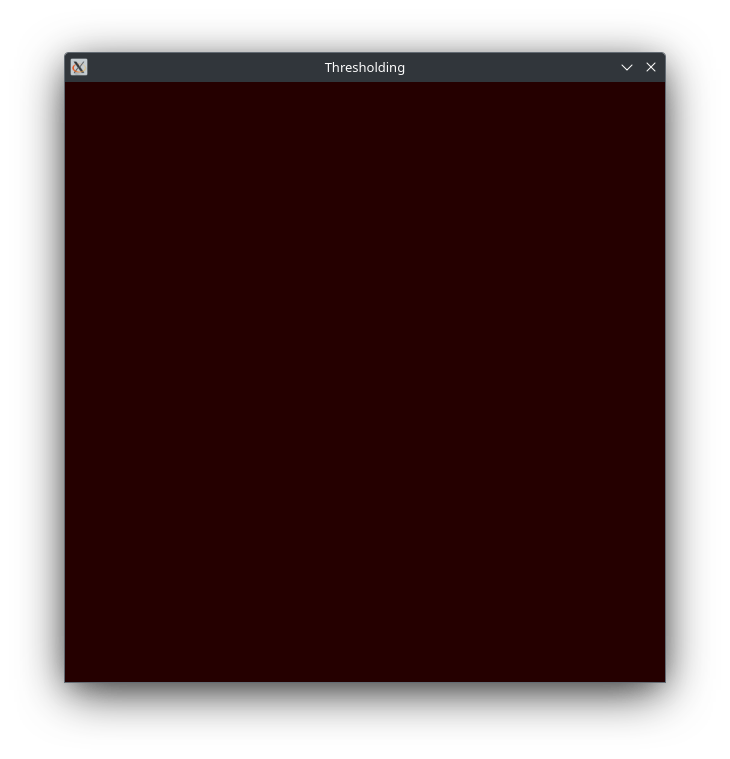
\includegraphics[width=0.25\textwidth]{./latex/img/m0}
    \end{multicols}
    \item Class [1,2]:
    \begin{multicols}{2}
        \begin{equation*}
            \begin{bmatrix}
                2 & 2 & 1 \\
                2 & 1 & 2 \\
                2 & 2 & 1
            \end{bmatrix}
        \end{equation*}
        \columnbreak
        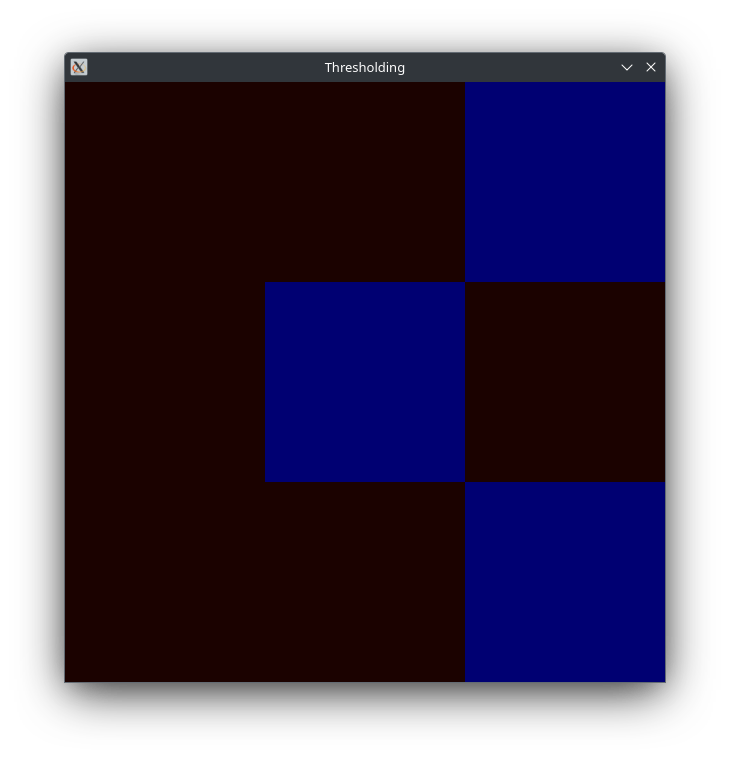
\includegraphics[width=0.25\textwidth]{./latex/img/m1}
    \end{multicols}
    \item Class [3,4,5,6]:
    \begin{multicols}{2}
        \begin{equation*}
            \begin{bmatrix}
                5 & 6 & 3 \\
                6 & 4 & 6 \\
                5 & 5 & 3
            \end{bmatrix}
        \end{equation*}
        \columnbreak
        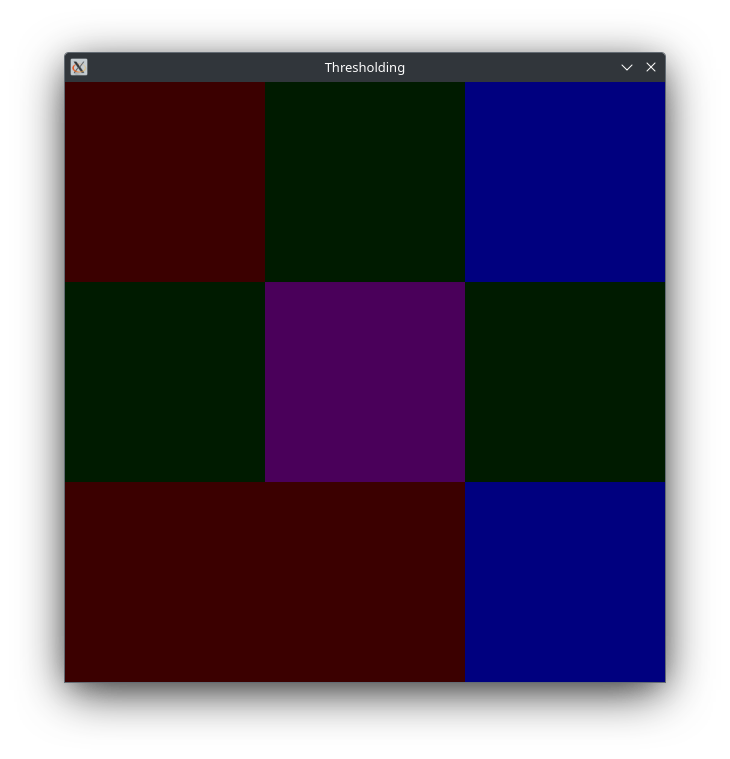
\includegraphics[width=0.25\textwidth]{./latex/img/m2}
    \end{multicols}
    \item Class [7,8,9,10,11,12]:
    \begin{multicols}{2}
        \begin{equation*}
            \begin{bmatrix}
                9  & 11 & 7  \\
                12 & 4  & 11 \\
                10 & 9  & 8
            \end{bmatrix}
        \end{equation*}
        \columnbreak
        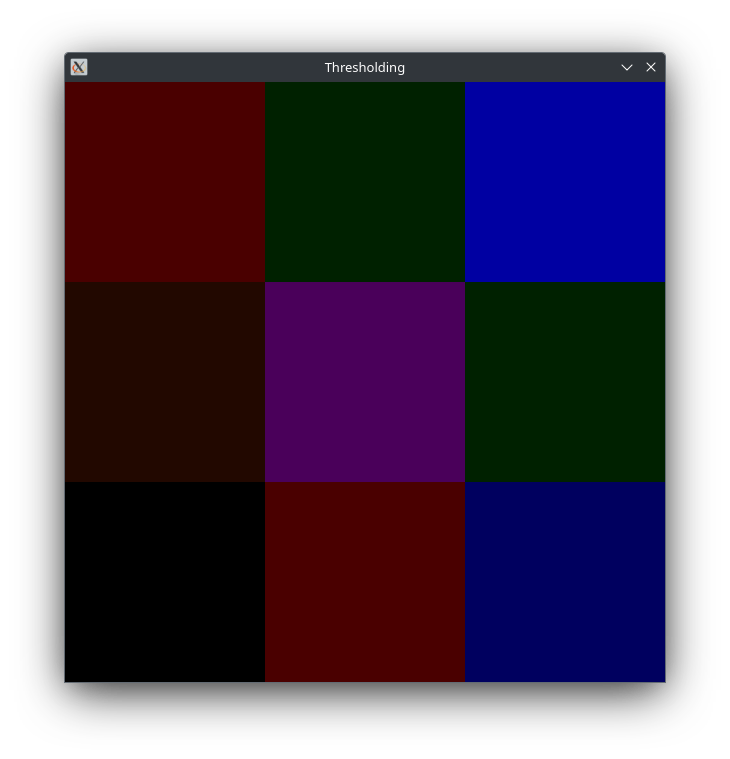
\includegraphics[width=0.25\textwidth]{./latex/img/m3}
    \end{multicols}
    \item Class [13,14,15,16]:
    \begin{multicols}{2}
        \begin{equation*}
            \begin{bmatrix}
                13 & 15 & 7  \\
                12 & 4  & 16 \\
                10 & 14 & 8
            \end{bmatrix}
        \end{equation*}
        \columnbreak
        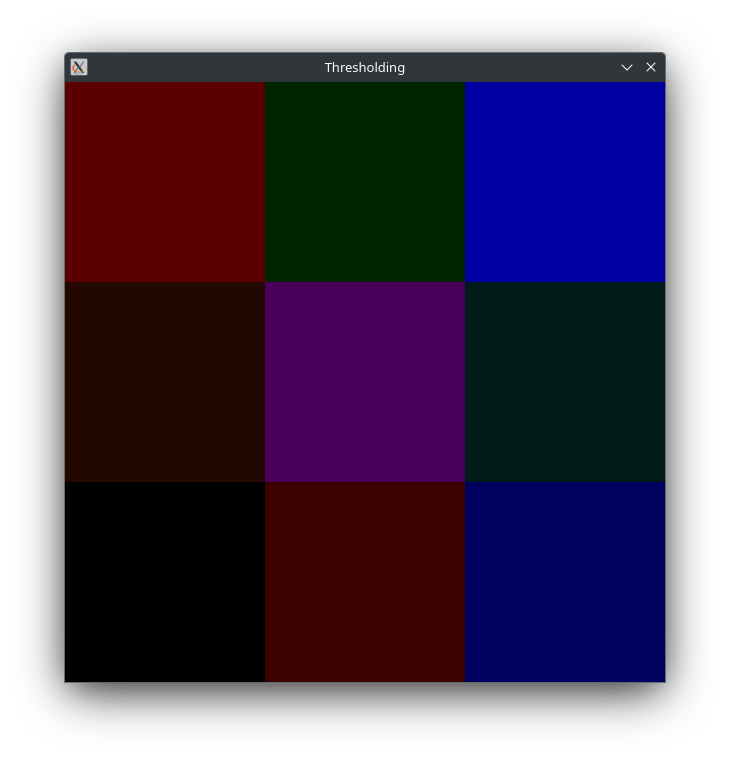
\includegraphics[width=0.25\textwidth]{./latex/img/m4}
    \end{multicols}
\end{enumerate}

Como podemos observar, el algoritmo converge en la cuarta iteración.
Debemos tener en cuenta que en una imagen de solo 9 píxeles (3x3), por lo que a lo sumo tendrá 9 clases diferentes, las cuales deben ser obtenidas en la cuarta iteración.
